\section{RESULTS} \label{sec:results}
\begin{figure}[htb]
\vspace{-10pt}
  \centering
    \subfigure[N/E localisation. High confidence in yaw measurement.] 			    
    {\label{fig:sim-straight2}
	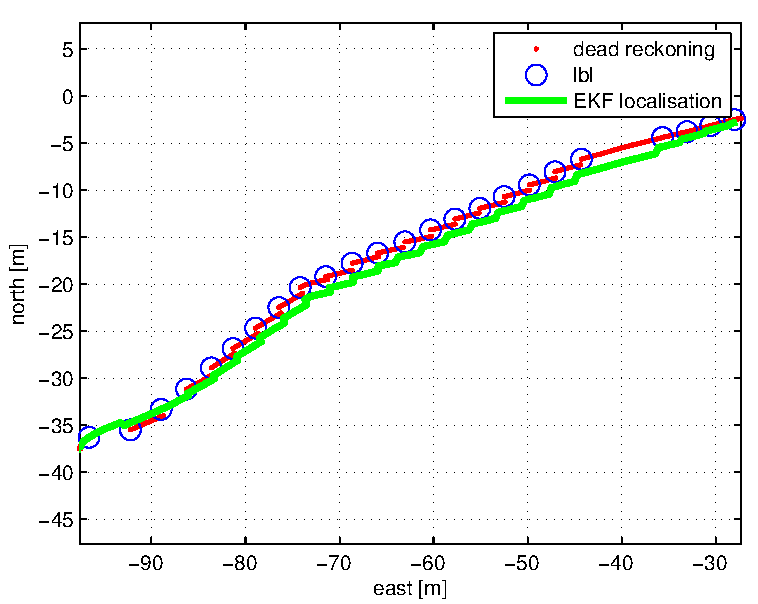
\includegraphics[width=0.7\linewidth]{sim-straight2.pdf}}
    \subfigure[N/E localisation. Confidence in yaw measurement lowered.] 
    {\label{fig:sim-straight1}
	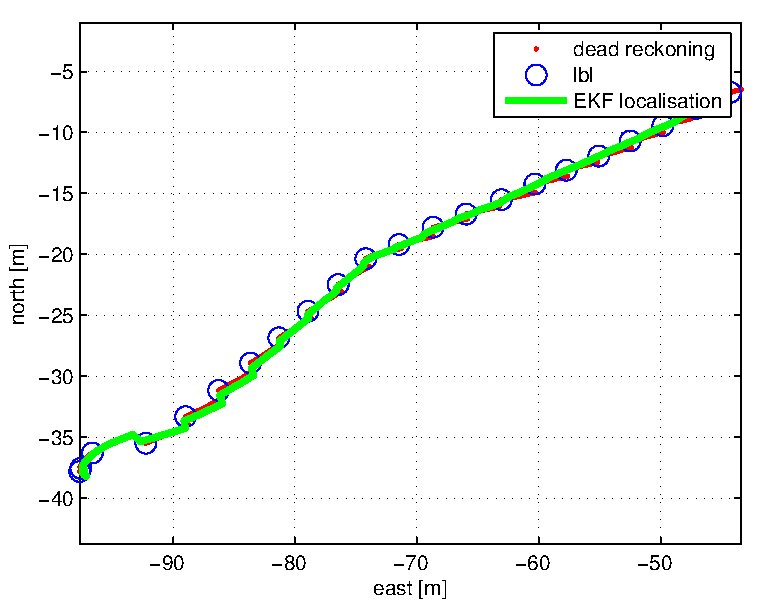
\includegraphics[width=0.7\linewidth]{sim-straight1.pdf}}   \\
    \subfigure[Heading estimation. Biased yaw measurement is being corrected by decreasing confidence in yaw measurement, SDyaw = 0.2$rad \approx 11.5 ^{\circ}$. SDyawRate = 0.004 $\frac{rad}{s}$.] 
    {\label{fig:yaw-straight1}
    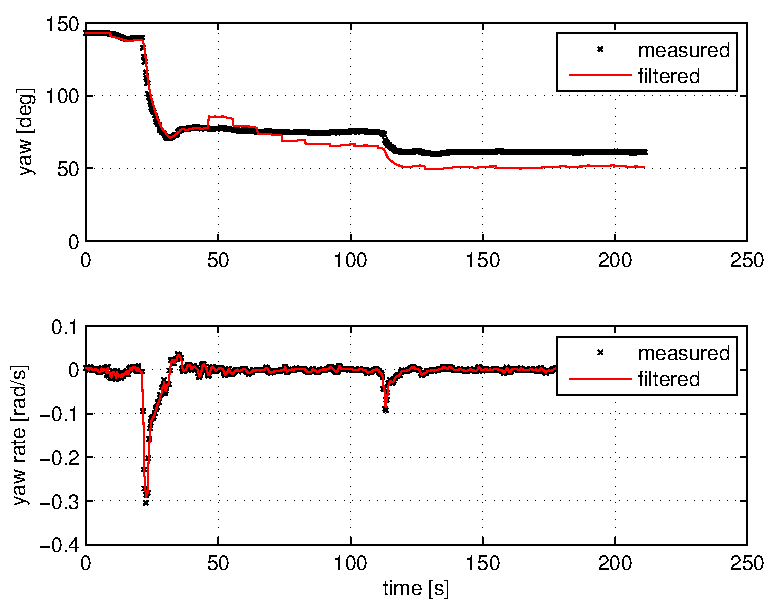
\includegraphics[width=0.8\linewidth]{yaw-straight1.pdf}}
\caption{AUV localisation using EKF. Yaw was measured by integrating yaw rate periodically measured using FOG.}
\vspace{-10pt}
\label{fig:auv-sim-straight}
\end{figure} 
Nessie missions were carried out as a part of the algorithm trials. It is useful to mention that there is no exact ground truth for underwater robot localization available. GPS signal, if available, could serve as an absolute position reference: either directly or in form of LBL. Experimental results have been obtained for different missions. Good news, however, is that the absolute depth measurement is quite accurate and frequent, making AUV localisation a 2D task.
%Selecting a heading measurement with good performance %, each option having different accuracy and performance. supplied with FOG-based INS, DVL and LBL,
For a high-end underwater vehicle such as Nessie, main source of navigation error is influenced by transformation of vehicle-referenced velocities to world-referenced velocities, particularly due to yaw (heading) measurement errors. Yaw can be measured directly using magnetic compass or integrating FOG-based yaw rates. Simulation with data from previous missions was carried out to see which device gives the best performance for a given underwater vehicle and possibilities of improvement using sensor fusion. Dead reckoning localisation substituted with occasional LBL position updates was compared with the localisation obtained after filtering (Figure ~\ref{fig:auv-sim-straight}) for the recorded straight line trajectory mission. 

Heading calculated by integrating FOG's yaw rate - tends to be accurate and fast, less prone to noise. Nevertheless, it is calculated each time by appending yaw rate value integrated in time on the previous yaw value (relative measurement). Therefore, it is sensible on initial absolute heading measurement. In case initial yaw is imprecise, a constant bias exists in yaw measurement (Figure ~\ref{fig:sim-straight2}). Thus, putting high trust in yaw measurement is not a recommendable strategy. Eventually, after assigning less confidence in yaw measurement (higher $\sigma_{yaw}$ value), bias becomes filtered out if measured and filtered heading are compared (Figure ~\ref{fig:yaw-straight1}).
% Biased yaw measurement not being corrected due to %low confidence in yaw measurement, SDyaw = 0.2$rad \approx 11.5 ^{\circ}$. SDyawRate = 0.004 $\frac{rad}{s}$, SDu/v = $1\frac{cm}{s}$.    
Tests show that localisation performance can be tailored by setting the confidence in prediction model or measurement values. Confidence is materialized as the variance of the random variable: the lower it is, more certain the value of the random variable is hence more confident in value of that variable we tend to be. EKF tries to optimise the result within the defined boundaries of uncertainty.
\begin{figure}%[htb]
  \centering
    \subfigure[N/E localisation.] {\label{fig:spiral2d}
	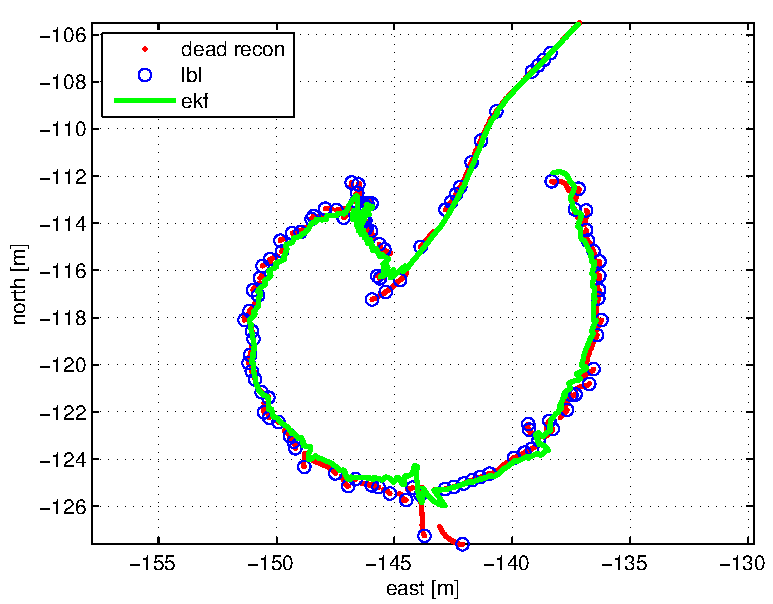
\includegraphics[width=0.7\linewidth]{spiral2d.pdf}}
    \subfigure[Depth.] {\label{fig:spiral-depth}
    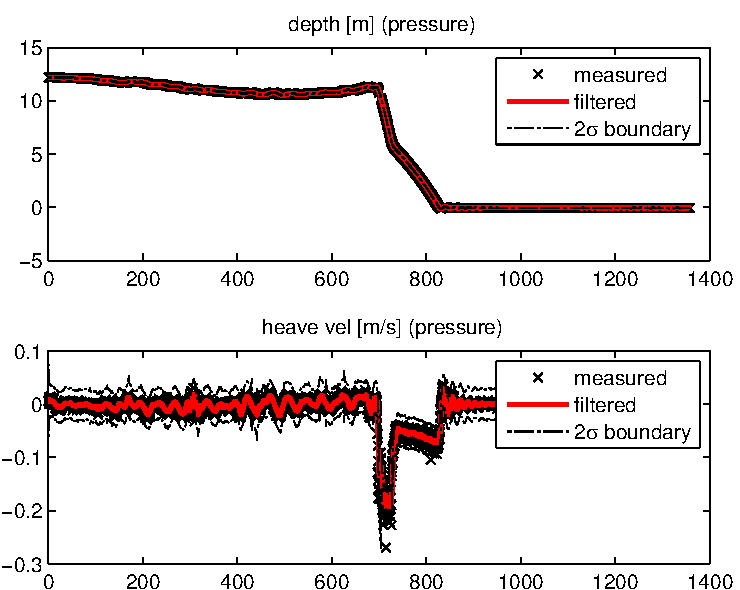
\includegraphics[width=0.7\linewidth]{spiral-depth.pdf}}
    \caption{Spiral trajectory and the trajectory estimation using EKF.}
    \label{fig:spiral}
\vspace{-10pt}
\end{figure}

Trajectory filtering is shown in example of spiral trajectory and surfacing action that was taken with Nessie starting from the depth of around 12 m. EKF estimation results are shown in Figure ~\ref{fig:spiral} together with LBL position updates and dead reckoning starting from each position. Similarly as with previous plots LBL-aided-dead reckoning was shown together with LBL position updates. Filtered trajectory does not experience severe jumps, and the curve seems to be smoother and less prone to drifting. Standard deviation of north and east measurement parameters was tested with different values, causing more or less confidence in LBL measurement hence shaping the localisation curve and managing filtering of the LBL outliers.  

Rectangular trajectories were tested in low depths of a lake, with the GPS signal available to be used as a position reference and ground truth indication (Figure ~\ref{fig:square-traj}). Dead reckoning navigation was used as a reference when controlling the vehicle movement during the experiment. This fact can cause slight confusion in analysis of the trajectory graphs since all the dynamics and forces were applied with respect to the dead reckoning navigation which is an estimated value. GPS signal available from the antenna located on the water surface is serving as a measure of absolute position within the lake - giving an idea about the actual vehicle position while it tries to moves within the boundaries of estimated dead reckoning position. Main issue when performing the square trajectory tests was significant imprecision of GPS signal (Figure ~\ref{fig:square}). GPS measurements were appended to the observations. EKF and UKF localisation results were shown in Figure ~\ref{fig:square} for $\sigma_{north}=\sigma_{east}=0.5m$. UKF was compared with the EKF localisation, under same parameter settings and using the real data obtained from Nessie sensors. Trajectory obtained using UKF tends to be slightly more precise compared with the one obtained using EKF. Since it is more precise algorithm when approximating nonlinearity \cite{julier96} , UKF preserves the formula of prediction model better.
\begin{figure}%[htb]
  \centering
    \subfigure[N/E localisation of a rectangular trajectory $(\sigma_{north} = \sigma_{east} = 0.5 m)$.] 
    {\label{fig:square}
	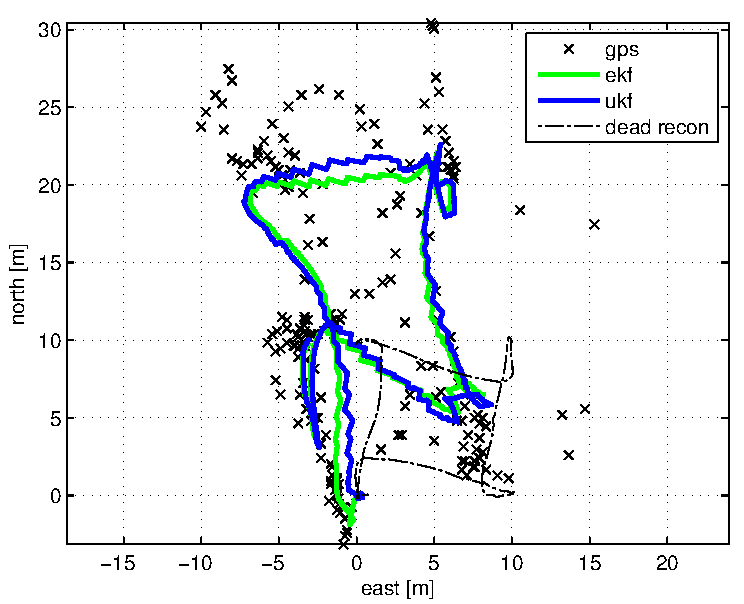
\includegraphics[width=0.7\linewidth]{square.pdf}} \\
    \subfigure[Filtered absolute position, linear velocities and heading recorded while making a rectangular trajectory.]  				{\label{fig:square-filtering}
    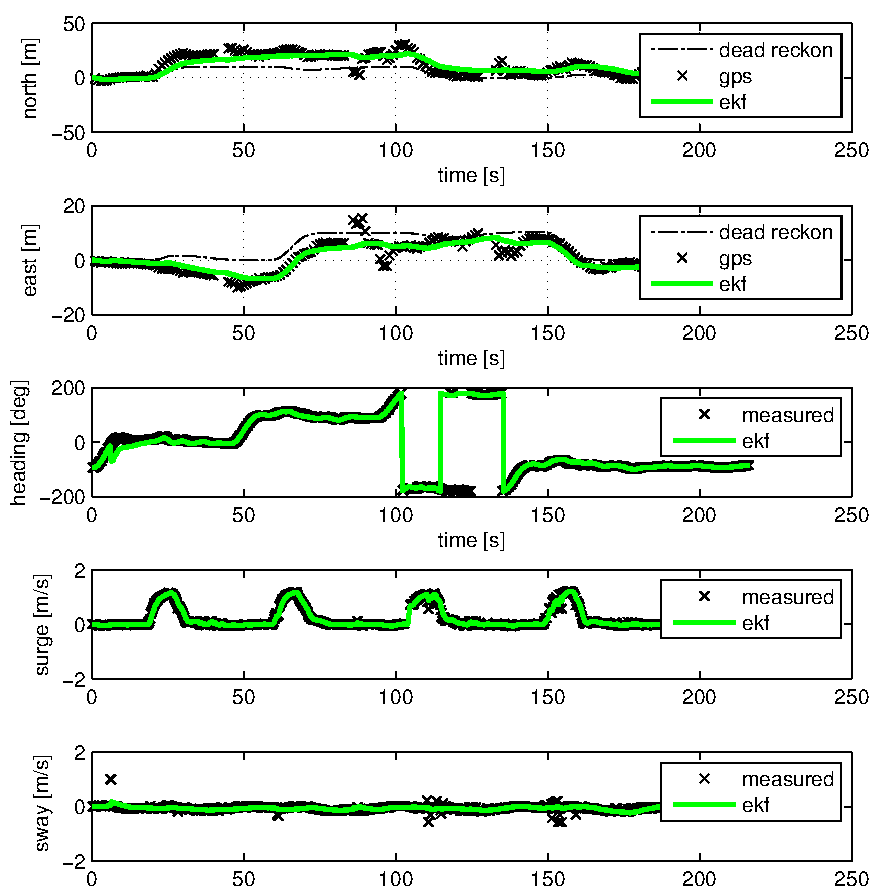
\includegraphics[width=0.98\linewidth]{square-filtering.pdf}}
\caption{GPS aided rectangular trajectory localisation using EKF and UKF.}
\label{fig:square-traj}
\vspace{-20pt}
\end{figure}
EKF tends to filter the GPS-measured north-east (N/E) coordinates, hence partially corrects the GPS imprecisions. At this point it is evident why EKF is a great tool. Filter tries to satisfy the set uncertainty boundaries and fuse all the available information trying to make the most out of it combined together in one mathematical system. Furthermore, fusing such imprecise and sketchy position data from GPS, still improves the localisation. Obtained trajectory tends to go towards what can be treated as expected path. From something that looked like a noisy collection of position observations at the beginning (Figure ~\ref{fig:square}), application of EKF together with sensor fusion enabled having generally better navigation performance.